\section{Auswertung}
\label{sec:Auswertung}
Die Fehlerrechnung des folgenden Kapitels wird mit Python durch Verwendung des Pakets \textit{uncertainties} \cite{uncertainties} durchgeführt.
Zur Berechnung der Theoriewerte müssen die Werte der Induktivitäten und der Kapazitätten der einzelnen Bauteile bekannt sein. Verwendet wurde 
die in \autoref{fig:Schaltung} gezeigte Schaltung mit den Werten 
\begin{align*}
    L &= 32.351 \, \unit{\milli\henry} & C &= 0.8015 \, \unit{\nano\farad} & C_{\text{Sp}} &= 0.037 \, \unit{\nano\farad}.
\end{align*}

\subsection{Einstellung der Resonanzfrequenz}
\label{subsec:A_Resonanz}
Wie in \autoref{subsec:Justierung} beschrieben, muss vor der eigentlichen Durchführung des Versuches die Resonanzfrequenz der Schwingkreise ermittelt und aufeinander abgestimmt 
werden. Für die Resonanzfrequenz des Schwingkreises ergibt sich der Wert $\nu^+ = 30.7 \, \unit{\kilo\hertz}$. Die theoretische Frequenz berechnet sich nach \autoref{eqn:T_nup}
durch Einsetzen von $C + C_\text{Sp}$ für die Gesamtkapazität zu $\nu^+_\text{Theorie} = 30.558 \, \unit{\kilo\hertz}$. Dies führt zu einer relativen Abweichung von 
$\symup{\Delta_\text{relativ}}(\nu^+) = 0.46 \, \%$. Die relative Abweichung eines Messwertes $x$ zu einem Theoriewert $x^*$ lässt sich dabei über den Zusammenhang
\begin{equation}
    \label{eqn:rel_Abw}
    \symup{\Delta_\text{relativ}}(x) = \frac{|x^* - x|}{x^*}
\end{equation}
berechnen.

\subsection{Bestimmung des Verhältnis der Perioden von Schwingung und Schwebung}
\label{subsec:A_Amplituden}
Die Messung zur Bestimmung des Amplitudenverhältnisses von Schwebung und Schwingung wurde bei einer Generatorfrequenz von $381 \, \unit{\hertz}$ durchgeführt.
Ein beispielhafter Graph des Oszilloskops ist in \autoref{fig:Amplituden} zu sehen. Eine Periode der Schwebung ist zwischen den roten Balken gekennzeichnet.
Fälschlicherweise wurden die Amplituden von je zwei Perioden gezählt, weshalb es durch die Mittelung auf eine Periodenlänge vorkommen kann, dass die Messwerte eine 
\dq halbe\dq \; Amplitude beinhalten.
\begin{figure}
    \centering 
    \caption{Anzeige des Oszilloskops unter Verwendung des $9.99 \, \unit{\nano\farad}$ Kondensators.}
    \label{fig:Amplituden}
    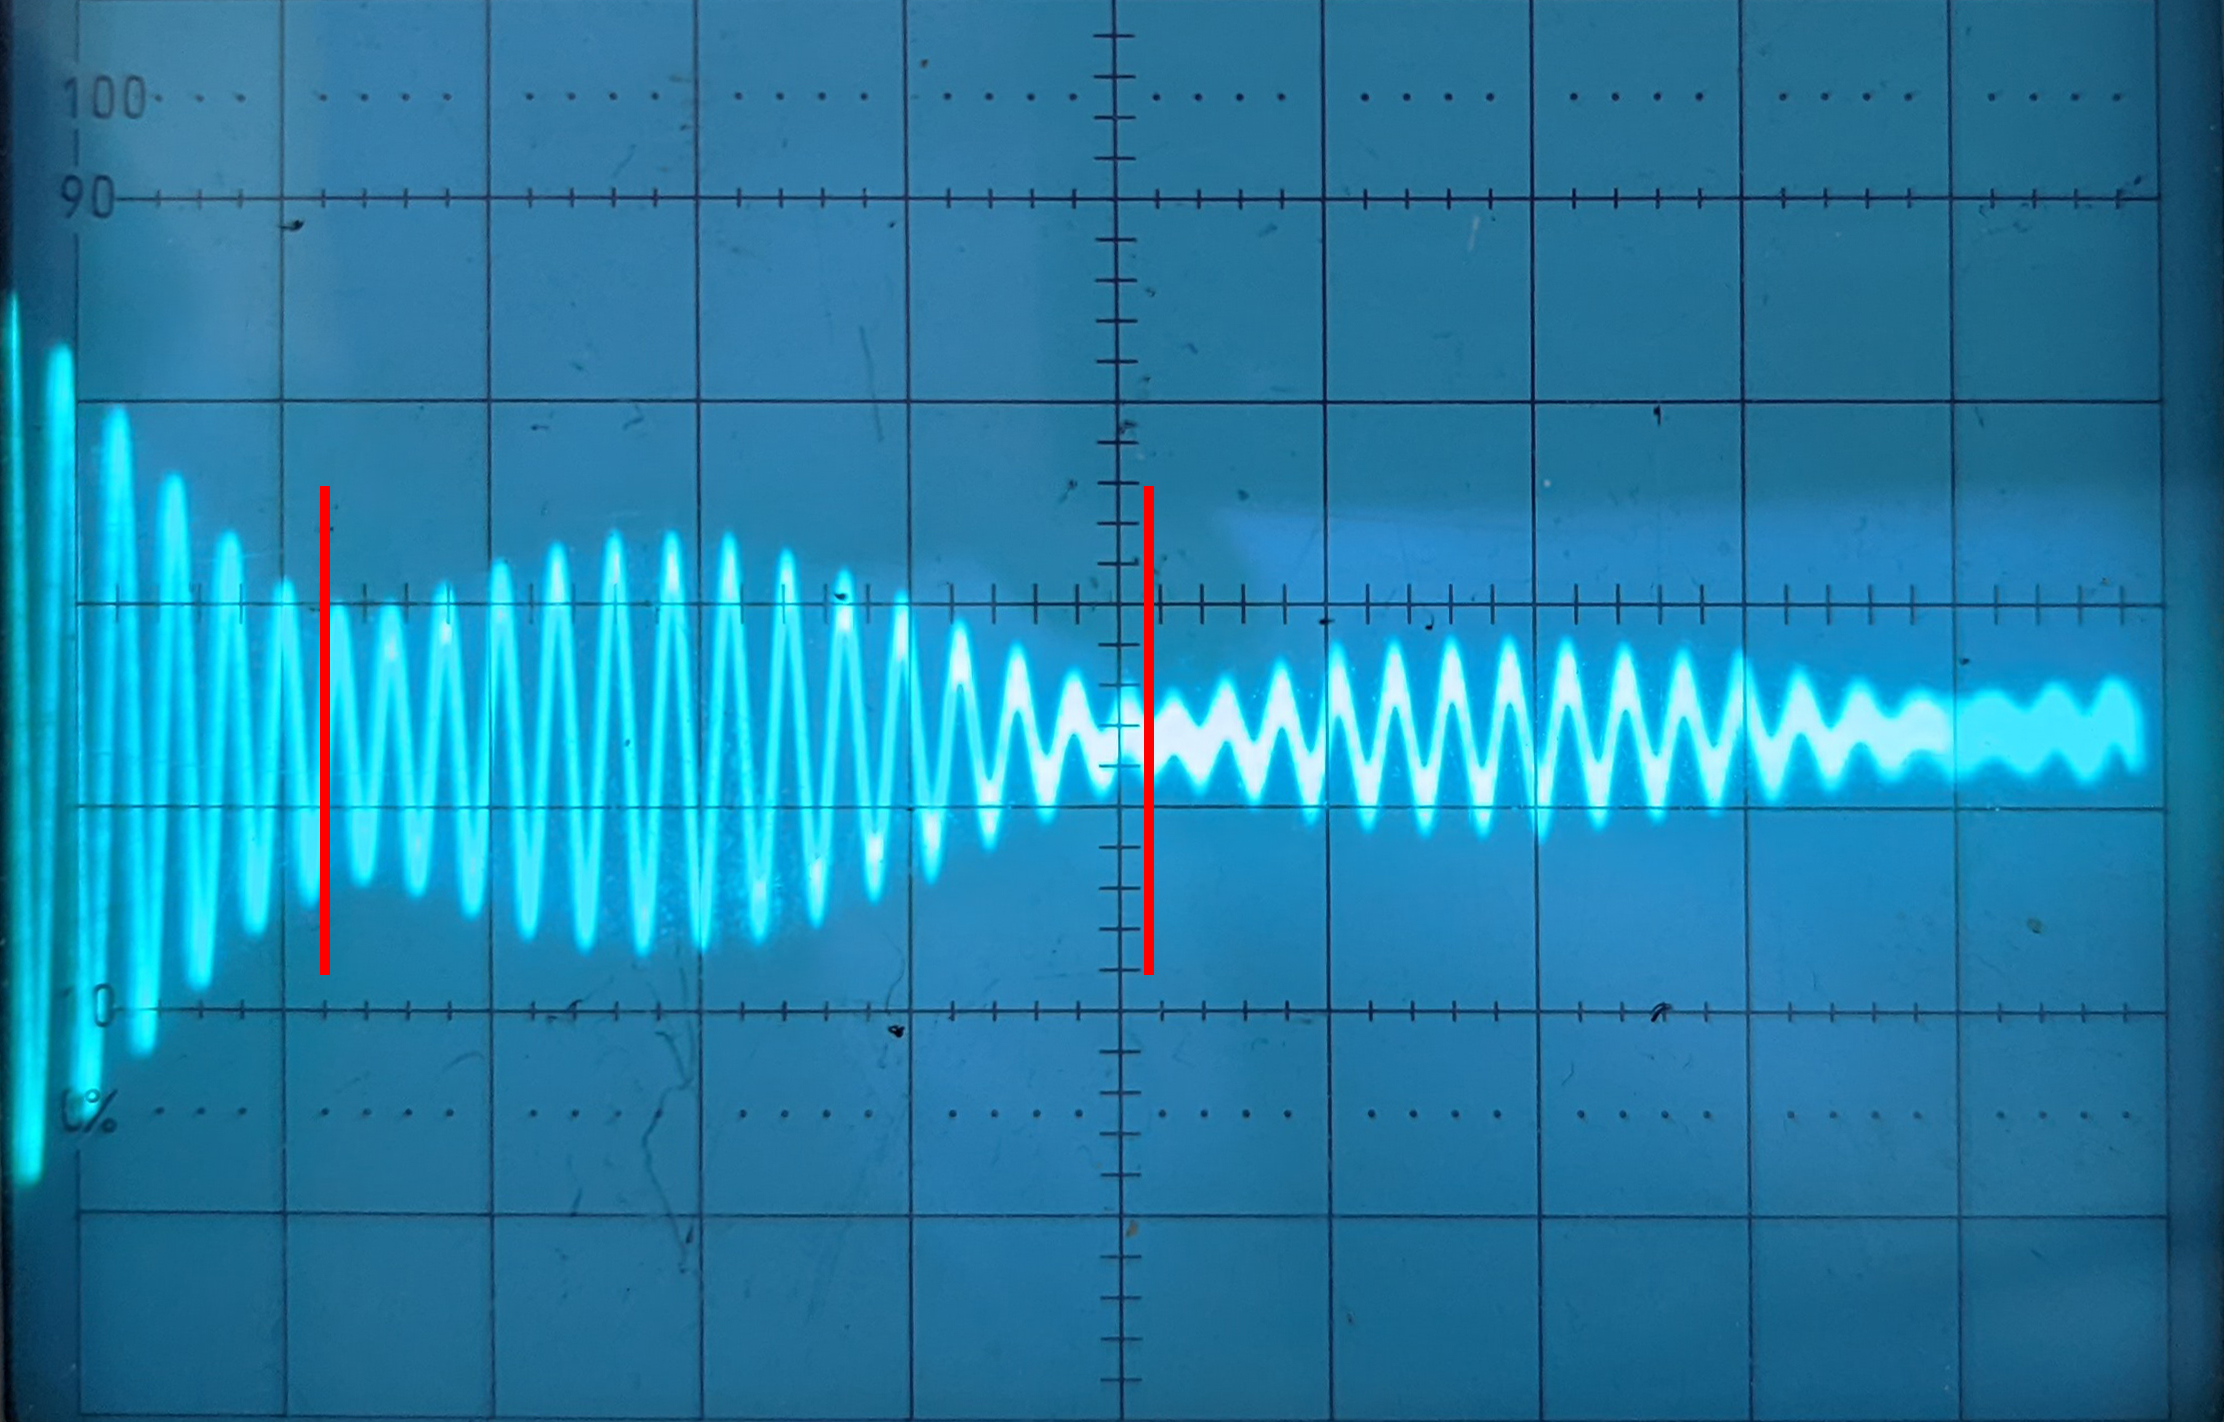
\includegraphics[width = 0.6\textwidth]{content/Amplituden.jpg}
\end{figure}

Zur Berechnung der Theoriewerte wird zunächst der Theoriewert der Frequenz $\nu^-$ unter Verwendung der \autoref{eqn:T_Schwebung} zu den jeweiligen Kondensatoren mit den Kapazitäten $C_\text{K}$ bestimmt. Auch hier muss 
die zusätzliche Kapazität der Spule $C_\text{Sp}$ berücksichtigt werden. Diese wird wie zuvor zusätzlich zur Gesamtkapazität addiert. Mittels der Werte von $\nu^+$ und $\nu^-$ 
lässt sich nach \autoref{T_Schwebung} die Frequenz der Schwebung berechenen, woraus wiederum das Verhältnis $n$ der 
Schwingungsperioden pro Schwebungsperiode nach \autoref{eqn:T_n} bestimmt werden kann. Die jeweiligen Werte können \autoref{tab:Werte_a} entnommen werden.
\begin{table}
    \centering
    \caption{Ergebnisse zur Messung des Verhältnisses von Schwingung und Schwebung} 
    \label{tab:Werte_a}
    \begin{tabular}{S[table-format=1.2] S[table-format=2.1] S @{${}\pm{}$} S[table-format=1.2] S[table-format=2.1]}
        \toprule 
        {$C_\text{K} \mathbin{/} \unit{\nano\farad}$} & {$n_\text{gemessen}$} & \multicolumn{2}{c}{$n_\text{Theorie}$} & {$\symup{\Delta_\text{relativ}}(n) \mathbin{/} \%$} \\
        \midrule
        9.99 & 14.0 & 14.1 & 0.04 &  0.8 \\
        8.00 & 12.0 & 11.5 & 0.03 &  4.2 \\
        6.47 & 10.5 &  9.5 & 0.03 & 10.4 \\
        5.02 &  8.5 &  7.6 & 0.02 & 11.7 \\
        4.00 &  7.0 &  6.3 & 0.02 & 11.6 \\
        3.00 &  6.0 &  5.0 & 0.01 & 21.0 \\
        2.03 &  4.5 &  3.7 & 0.01 & 22.5 \\
        1.01 &  3.0 &  2.3 & 0.00 & 30.3 \\
        \bottomrule 
    \end{tabular}
\end{table}

\subsection{Bestimmung der Fundamentalfrequenzen über Lissajous-Figuren}
\label{subsec:A_Messung_b}
Die Theoriewerte der Fundamentalfrequenzen $\nu^+$ und $\nu^-$ wurden bereits bestimmt. Mithilfe der Lissajous-Figuren lassen sich Messwerte für diese Frequenzen experimentell 
bestimmen, die \autoref{tab:Werte_b} entnommen werden können. Der Theoriewert der Frequenz $\nu^+$ ist konstant und gegeben durch 
$\nu^+_\text{Theorie} = 30.558 \, \unit{\kilo\hertz}$.
\begin{table}
    \centering
    \caption{Mess- und Theoriewerte und dazugehörige Abweichungen der Fundamentalfrequenzen bei Bestimmung über Lissajous-Figuren.} 
    \label{tab:Werte_b}
    \begin{tabular}{S[table-format=1.2] S[table-format=2.2] S S S @{${}\pm{}$} S[table-format=1.3] S[table-format=2.2]}
        \toprule
        {$C_\text{K} \mathbin{/} \unit{\nano\farad}$} & {$\nu^+_\text{exp} \mathbin{/} \unit{\kilo\hertz}$} & {$\symup{\Delta_\text{rel}}(\nu^+) \mathbin{/} \% $} &%
        {$\nu^-_\text{exp} \mathbin{/} \unit{\kilo\hertz}$} & \multicolumn{2}{c}{$\nu^-_\text{Theorie} \mathbin{/} \unit{\kilo\hertz}$} &%
        {$\symup{\Delta_\text{rel}}(\nu^-) \mathbin{/} \%$} \\
        \midrule
        9.99 & 31.26 &  2.29 & 32.94 & 32.80 & 0.006 & 0.42 \\
        8.00 & 31.40 &  2.76 & 33.47 & 33.33 & 0.008 & 0.41 \\
        6.47 & 31.58 &  3.34 & 34.08 & 33.95 & 0.010 & 0.39 \\
        5.02 & 31.83 &  4.16 & 34.98 & 34.85 & 0.012 & 0.36 \\
        4.00 & 32.11 &  5.08 & 35.97 & 35.85 & 0.014 & 0.33 \\
        3.00 & 32.58 &  6.62 & 37.51 & 37.41 & 0.018 & 0.26 \\
        2.03 & 33.42 &  9.37 & 40.25 & 40.19 & 0.025 & 0.16 \\
        1.01 & 35.83 & 17.25 & 47.38 & 47.52 & 0.039 & 0.29 \\
        \bottomrule 
    \end{tabular}
\end{table}

Betrachet man die Messwerte der Frequenz $\nu^+$ fällt auf, dass diese stetig ansteigen, obwohl sie theoretisch konstant sein sollten. Ein Grund dafür könnte ein systematischer
Fehler sein, da die eigentliche Frequenz von $\nu^+$ auf $30.7 \, \unit{\kilo\hertz}$ eingestellt wurde und sich bei ungefähr diesem Wert auch eine Gerade der Lissajous-Figuren 
ergab. Die Werte, an denen diese Gerade auftritt wurden bedauerlicherweise nicht notiert, jedoch lagen diese nahe bei der eingestellten Resonanzfrequenz. Die Ursache für das
Auftreten der Geraden zwischen der Resonanzfrequenz und der Frequenz $\nu^-$ ist unklar.

\subsection{Bestimmung der Fundamentalfrequenzen mittels der \textit{Sweep}-Funktion}
\label{subsec:A_Messung_c}
Bei dieser Messung wird die \textit{Sweep}-Funktion des Spannungsgenerators verwendet. Der Startwert des Frequenzspektrums wurde vor der Messung auf $20 \, \unit{\kilo\hertz}$ 
eingestellt. Am Ende der Messreihe lag die Einstellung jedoch bei $19.7 \, \unit{\kilo\hertz}$. Der Endwert des Spektrums wurde auf $50 \, \unit{\kilo\hertz}$ geregelt und lag 
am Ende der Messreihe bei $49.4 \, \unit{\kilo\hertz}$. Die Zeit in der das Spektrum durchlaufen wird wurde auf $0.02 \, \unit{\second}$ eingestellt.
Die Zeitpunkte, an denen die Peaks der Frequenzen $\nu^+$ und $\nu^-$ auftreten lassen sich mit Hilfe einer linearen Funktion in die jeweiligen Frequenzen umrechenen, da die
\textit{Sweep}-Funktion des Spannungsgenerators das Frequenzspektrum linear durchläuft. Die Breite $b$ des Frequenzspektrums liegt für alle Kopplungskondensatoren konstant 
bei $b = 11 \, \unit{\micro\second}$. Auch der Zeitpunkt, an dem die Frequenz $\nu^+$ auftritt ist konstant an der Stelle $t^+ = 4.4 \, \unit{\micro\second}$, was einer 
Frequenz von $\nu^+_\text{exp} = 31.58 \, \unit{\kilo\hertz}$ entspricht, die um $3.34 \%$ vom Theoriewert $\nu^+_\text{Theorie} = 30.558 \, \unit{\kilo\hertz}$ abweicht.
Die Messwerte zu der Frequenz $\nu^-$ sind \autoref{tab:Werte_c} zu entnehmen.

\begin{table}
    \centering
    \caption{Mess- und Theoriewerte und dazugehörige Abweichungen der Fundamentalfrequenz $\nu^-$ bei Bestimmung mithilfe der Sweep-Funktion.} 
    \label{tab:Werte_c}
    \begin{tabular}{S[table-format=1.2] S[table-format=1.1] S[table-format=2.2] S @{${}\pm{}$} S[table-format=1.3] S[table-format=1.2]}
        \toprule
        {$C_\text{K} \mathbin{/} \unit{\nano\farad}$} & {$t^-_\text{exp} \mathbin{/} \unit{\micro\second}$} &%
        {$\nu^-_\text{exp} \mathbin{/} \unit{\kilo\hertz}$} & \multicolumn{2}{c}{$\nu^-_\text{Theorie} \mathbin{/} \unit{\kilo\hertz}$} &%
        {$\symup{\Delta_\text{rel}}(\nu^-) \mathbin{/} \%$} \\
        \midrule
        9.99 & 5.2 & 33.74 & 32.80 & 0.006 & 2.86 \\
        8.00 & 5.6 & 34.82 & 33.33 & 0.008 & 4.46 \\
        6.47 & 5.8 & 35.36 & 33.95 & 0.010 & 4.16 \\
        5.02 & 6.0 & 35.90 & 34.85 & 0.012 & 3.00 \\
        4.00 & 6.2 & 36.44 & 35.85 & 0.014 & 1.64 \\
        3.00 & 7.0 & 38.60 & 37.41 & 0.018 & 3.17 \\
        2.03 & 8.0 & 41.30 & 40.19 & 0.025 & 2.77 \\
        \bottomrule 
    \end{tabular}
\end{table}
Zu dem Kopplungskondensator mit Kapazität $C_\text{K} = 1.01 \, \unit{\nano\farad}$ konnten keine experimentellen Werte bestimmt werden, da auf Grund der Auflösung des Oszilloskops
kein genaues Ablesen der Messwerte möglich war.
